\section{\mc EEGの測定}
\subsection{特徴}
ヒトの脳活動計測によって獲得したいものは、精神活動・行動の生物学的基盤となる
脳の神経活動である。その最小単位は百億とも二百億とも言われる脳の神経細胞(ニューロン)の
電気的活動だが、個々のニューロンの活動を非侵襲的に計測する事は不可能である。
しかし、ニューロンの活動に伴って様々な生理現象が生ずる。
まずニューロンが電気的な活動(一次信号)を行うためにはエネルギーを必要とし、
糖の分解のための代謝活動(二次信号)が生ずる。酸素と糖は脳にはほとんど貯蔵されていないため、
代謝活動に伴ってエネルギーを必要としている脳の部位に関して、局所脳血流(三次信号)が増大する。
非侵襲計測では一次信号から三次信号のいずれかを計測し、
その信号の空間的・時間的なパターンから神経活動が生じた脳の部位及び時間を推定することで、
ヒトの脳活動を計測する。EEGやMEGは脳の電気的な活動である一次信号を計測しており、
fMRIやNIRSは血流に関する三次信号を計測している(図\ref{fig:信号フロー}\cite{脳を測る})。
\begin{figure}
    \centering
    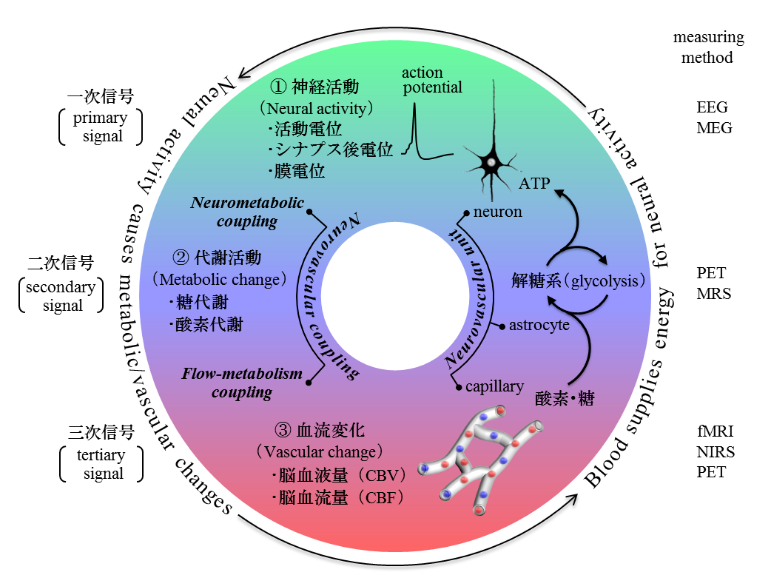
\includegraphics[width=15cm]{images/signalflow.png}
    \caption{一次信号、二次信号、三次信号と計測方法の関係図\cite{脳を測る}}
    \label{fig:信号フロー}
\end{figure}

EEGは一次信号を計測したものであるためNIRSやfMRIに比べ脳活動に対する測定値の遅れは
少ない。また非侵襲計測の中では最も時間分解能が高いとされる。
ここで時間分解能とは脳の同一の場所が短時間に二回活動した場合に、
それぞれを時間的に独立した脳活動として計測できる最短の時間間隔である。
一方で頭蓋骨や皮膚、毛髪などは電位にとっては透明ではないため空間分解能は低いとされる。
ここで空間分解能とは脳の異なる部位が同時に二箇所活動した場合に、それぞれを活動部位が異なる
独立した脳活動として計測できる最小の距離である。

ただし、通常の計測においては計測装置の空間分解能や時間分解能は測定対象には依存しないが、
脳活動計測の場合においては一般的に計測対象としている現象の時空間特性や脳活動の強さ、
あるいは発生源が皮膚表面であるか脳の深部であるかなどにも依存する。
従って、EEGを計測する場合、電極の数を増やして頭皮上に密に配置しサンプリングレートを上げれば
計測機器としての空間分解能や時間分解能を上げることはできるが、
脳活動計測としては必ずしも分解能が同様に向上するとは限らない。

\subsection{計測対象}
脳活動時にはシナプス活動によるシナプス後電位の発生に伴って
大脳皮質の錐体細胞の細胞体と尖端樹状突起の間で細胞内電流が流れる。
細胞内電流は細胞外へ流れ出て、細胞内へ戻る帰還電流を形成する。
また、興奮性シナプス後電位の空間的・時間的荷重によってニューロンが脱分極し、
神経線維を伝搬する活動電位もあるが持続時間が短いため、同期的荷重が起こりにくく、
一部の例外を除いてEEGの発生には寄与しないと考えられている。
従って、EEGで計測される脳活動は、ある領域からの出力(活動電位)よりもシナプスを介した
その領域への入力と領域内でのニューロンの結合による領域内の信号処理を強く反映していると考えられる。

いずれにせよ個々のニューロンが発生する電流は極めて小さいが、錐体細胞は皮質表層に向かって
尖端樹状突起が垂直に伸び、各細胞が平行に並んでいるため、多数の錐体細胞が同期して活動すれば、
頭外部から観測可能な電流源となる。
EEGは主に細胞が帰還電流によって生じる頭皮上での電位差を電極によって計測していると考えられている。
EEGの周波数帯域は1Hz以下から数十Hz、さらに数百Hzの成分も報告されている。

